\documentclass[a4paper,10pt]{article}

\usepackage[utf8]{inputenc}
\usepackage[T1]{fontenc}
\usepackage[french]{babel}
\usepackage{float}
\usepackage{afterpage}
\usepackage[backend=bibtex]{biblatex}
\usepackage{graphicx}
\bibliography{definition}

\usepackage{hyperref}

\title{Régulation d'un système dynamique : application à une serre}
\author{A. Caccia \and A. Madeira Cortes \and N. Marchant \and R. Fontaine}
\date{ }

\begin{document}

\maketitle

\vspace{1cm}

\section{Sujet}

Le but du projet est de modéliser et gérer dynamiquement l'environnement d'une serre. Plusieurs variables seront mesurées et devront être maintenues dans des bornes acceptables pour les plantes: humidité du sol et de l'air, luminosité et température. Ces variables seront mesurées grâce des capteurs installés dans la serre. \\

Lorsque ces variables dépassent des bornes supérieure ou inférieure acceptables, le logiciel développé activera des dispositifs pour les rétablir entre ces bornes. C'est à dire: \\

\begin{enumerate}
	\item la température est régulée par une résistance chauffante et un ventilateur,
	\item l'humidité de l'air est régulée par un brumisateur et le ventilateur,
	\item l'humidité de du sol est régulée par un système d'irrigation,
	\item la luminosité est régulée par une lampe et un système de volets.\\
\end{enumerate}

\newpage

\section{Implémentation}

Le projet sera implémenté en plusieurs parties :

\begin{enumerate}
    \item la mesure des variables du système,
    \item le filtrage de ces mesures,
    \item l'algorithme de contrôle en lui-même (probablement PID, voir \cite{Kinnaert2013}),
    \item l'exécution des commandes de correction (déterminées à l'étape précédente) par le matériel.
\end{enumerate}

La mesure de l'état du système sera fait à l'aide d'un Arduino et de capteurs analogiques simples à notre disposition à UrLab (le hackerspace de l'ULB). L'Arduino transmettra ensuite ces valeurs à un ordinateur qui filtrera celles-ci pour les donner en entrée à l'algorithme de contrôle. Ce dernier enverra ensuite des ordres au matériel (ventilateur, humidificateur, ...) qui seront eux aussi connectés à un Arduino.

Selon les résultats obtenus avec un PID simple, nous pourrions implémenter plusieurs variantes de PID ainsi que d'autres algorithmes de contrôle pour comparer leurs avantages et inconvénients.


\section{Dispositif de présentation au Printemps des Sciences}

Lors du Printemps des Sciences, nous envisageons de présenter notre projet en exposant une serre où sont cultivées des fraises. Il est aussi envisagé d'exposer une plus grande serre que Inforsciences nous prêterait.

Pour rendre la présentation dynamique et interactive, nous pourrions volontairement perturber le système et celui-ci se stabiliserait tout seul. Nous pourrions par exemple :
\begin{enumerate}
	\item allumer une lampe et qu'en réaction le système ferme les volets,
	\item chauffer la serre avec un dispositif externe (par exemple, un sèche-cheveux) pour que la ventilation s'enclenche,
	\item autres.
\end{enumerate}


Pour rendre l'expérience plus visuelle, nous pouvons aussi afficher en temps réel des graphes des données ainsi que les consignes de contrôle données au matériel. Pour cela, nous envisageons d'utiliser Grafana, un outil libre de visualisation de données temporelles. Il serait possible d'afficher un historique avec des bornes délimitées (en bleu et rouge sur la figure suivante). \\

\thispagestyle{empty}
\begin{figure}[H]
\centering
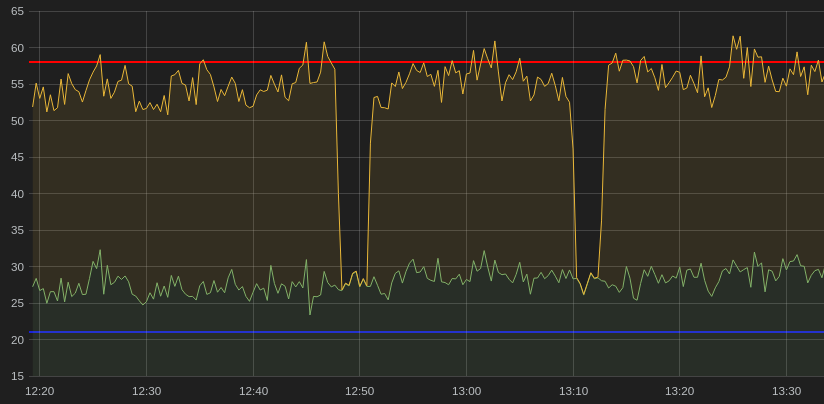
\includegraphics[scale=0.5]{figures/Grafana.png}
\caption{Grafana affichant des données temporelles}
\label{grafana}
\end{figure}


\section{Sources utilisées}

Pour commencer, nous nous baserons sur des cours d'automatique détaillant les bases de la théorie du contrôle et plus particulièrement de l'algorithme PID. Ceux-ci sont les cours ``MATH-H-304 - Automatique'' \cite{Kinnaert2013} dispensé à l'École Polytechnique de l'ULB et le cours dispensé à Caltech : ``Control System Design'' \cite{Knospe2006}. \\

Nous ferons un rapprochement avec un cas d'étude assez proche du notre : le contrôle de la température dans une serre, \citetitle{Zheying2014} \cite{Zheying2014} dans lequel les auteurs utilisent une version ``fuzzy'' de l'algorithme PID.

Ensuite, nous utiliserons deux documents détaillant des implémentations matérielles et logicielles proches de notre but: \citetitle{Ioannidis2014} \cite{Ioannidis2014} qui utilise un Raspberry Pi et \citetitle{ATMEL2005} \cite{ATMEL2005} qui utilise un microcontrôleur AVR. \\

Pour étudier des variantes à l'algorithme PID, nous nous référerons à \citetitle{Afou2014} \cite{Afou2014}, \citetitle{ballard1993pid} \cite{ballard1993pid} et \citetitle{Saletovi2014} \cite{Saletovi2014} \\

Parallèlement au problème du contrôle, nous envisageons d'utiliser des filtres de Kalman pour filtrer le signal en entrée de PID pour ne pas amplifier le bruit des capteurs et éventuellement prédire l'état futur du système. Pour cela, nous nous baserons sur l'article \citetitle{Welch2006} \cite{Welch2006}.

\newpage

\printbibliography

\end{document}
